\documentclass{article}
\usepackage{graphics, verbatim, multicol}

\newcommand{\titleize}[1]{\mbox{}\\ \Large \textsc{#1} \normalsize}

\newcommand{\headerstuff}{
%\begin{center}
\titleize{Alpheus Madsen} \\

\rule{1in}{.01in} \\

(435)764-5172 \\

alpheus.madsen@gmail.com \\

\rule{4in}{.01in}
%\end{center}
}

\newcommand{\sectionline}{
\begin{center}
   \rule{1in}{.01in}
\end{center}
}

\title{A Simple 3D Graphics Engine}
\author{\headerstuff}
\date{}

\begin{document}
\maketitle

This is the source code of a program I wrote during my first summer as a graduate student.  This program relies Allegro 4.2.2 (a computer game library downloadable at ``http://alleg.sourceforge.net'') and Alpy 0.1.3 (Python bindings for Allegro; this makes it possible to use some of Allegro's functions under Python; it can be downloaded at ``http://pyallegro.sourceforge.net'', although you need to scroll down and click on the link ``SourceForge file section'' in the section ``Alpy 0.1.3 released''---note that this program does not seem to work under Alpy 0.1.5).  I chose to write this program in Python because Python is a powerful yet easy-to-learn scripting language that can be mixed relatively easily with C or C++.  These features make Python ideal as a prototyping language.

It should be noted that I have only attempted to use this program under Linux; I have no idea how well it would run under other operating systems.

\begin{figure}
   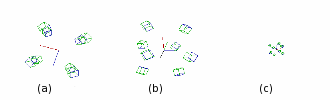
\includegraphics{screenshots4.png}
\caption{Three screen shots from ``littlecubesystem.py'': (a) rotation of system around the $z$-axis, (b) rotation of system around the vector $(5, 5, 2)$, and (c) camera ``rides away'' from the system.}\label{screenshots}
\end{figure}

My program implements a 3D camera, draws a coordinate axis for reference, and then draws eight cubes being rotated around different rotational axes.  (The rotations are implemented through quaternion multiplication.)  In addition to rotating the cubes individually, the entire system is rotated around the $x$-axis.  By pressing any key, the rotational axis is switched to the $z$-axis, then the $y$-axis, and finally the unit vector in the direction of the vector $(5, 5, 2)$; another press then ``freezes'' the system (while the cubes continue to rotate), and a final press then causes the camera to ``ride away'' from the system.  (Figure~\ref{screenshots} shows some screen shots.)

Having completed my camera apparatus, I had hoped to make a wireframe chess piece, and then expand my 3D engine to include the following:
\begin{itemize}
   \item Filling in of faces, and establishing appropriate drawing orders;

   \item Clipping and ``distance fog'', to limit the number of polygons needed to write to the screen;

   \item A physics engine, to realistically represent momentum, inertia, gravity, rotational momentum, and so forth;

   \item Ability to move characters using a keyboard or joystick.

   \item Re-implementation of the classes to make objects easier to manipulate;

   \item Re-implementation of crucial portions in C++, to increase the speed of the program.
\end{itemize}
In particular, I hope to expand this engine to become a computer game.  My goals in this regard were delayed as my graduate studies intensified.

Since high school I have always been interested in programming computer games.  It is a little unfortunate that my interest began in a time when 3D game engines were coming of age; my ``career'' wouldn't be able to mature with the industry.  I couldn't start my career with a simple yet popular game like Pong (that, despite its simplicity, taxed the available computing resources at the time) and continue writing more complex programs, eventually leading up to Doom III.  Instead, I have the desire (and the far more difficult goal) to write a full-fledged 3D computer game!

Even so, I have always had an affinity with writing 3D programs; this field fuses together computer programming with linear algebra in a concrete, visual way.  Due to my studies as a graduate student, however, and the complexities of the project, I simply have not had the time to pursue this project as much as I would have liked.

%\newpage

\sectionline

The file ``math3d.py''.  This module conveniently brings together all the modules I wrote for my 3D graphics engine.  It's rather boring!  I decided to put it first, as a sort-of table of contents of the rest of the modules.

\verbatiminput{math3d.py}

% \newpage

\sectionline

In the module ``ttable.py'', I define special trigonometric functions that rely on table lookups rather than direct computation; I use ``bradians'' as an alternative to radians or degrees to take advantage of the binary nature of computers:  one byte will contain all possible bradian values.

\verbatiminput{ttable.py}

%\newpage

\sectionline

The module ``vertex.py'' contains everything convenient for working with vertices (represented as vectors), edges and faces.  I first define the vector class and vector algebra, then go on to define edges and faces, and end by defining two useful ``palettes'' of colors.

\verbatiminput{vertex.py}

% \newpage

\sectionline

The next module, ``matrix.py'', defines some matrix algebra, and produces various matrices (including camera matrices) that would be useful in working with computer graphics.

\verbatiminput{matrix.py}

% \newpage

\sectionline

The next module, ``movable.py'', creates the class that is the foundation for all my 3D objects.

\verbatiminput{movable.py}

% \newpage

\sectionline

The module ``wf.py'' provides the class that reads in data files and uses them to create wireframe objects.

\verbatiminput{wf.py}

% \newpage

\sectionline

This next module, ``camera.py'', defines two different cameras that could be used to render a scene.  This is the core of the 3D graphics engine.

\verbatiminput{camera.py}

% \newpage

\sectionline

The file ``littlecubesystem.py''.  It uses my camera, as implemented in the previous modules, and displays the rotating cubes.

\verbatiminput{littlecubesystem.py}

% \newpage

\sectionline

The data file ``littlecube.dat'' contains the information needed to create a cube.  The comments in this file also explain how to write (or generate via software) other wireframe files.

\verbatiminput{littlecube.dat}

% \newpage

\sectionline

This data file, ``coords.dat'', provides the coordinate axis that is drawn by the program.

\verbatiminput{coords.dat}

% \newpage

\sectionline

For completeness, the data for the bradian sine table, ``sintable.dat'' is also provided; this is a computer-generated file.  It starts with the bradian sine of $0$, and then increments up to the bradian sine of $255$.

In the original text file, these numbers are in a single column; to save space (and to make it more readable), these numbers are shown here in three columns.

\begin{multicols}{3}
\verbatiminput{sintable.dat}
\end{multicols}

\end{document}
